\subsection{Introducing strings}
The point of basic patterns is to use them in more complex systems
with an understanding of the resulting behavior.  Imagine a string 
of characters in an alphabet a, b, and c.  The grammar evolved to 
have more constants 
\begin{center}
\begin{gcode}[]
<abc> ::=  
       | a <abc> 
       | b <abc>
       | c <abc> 
\end{gcode}
\end{center}
So this grammar accepts \emph{aabaabcac} 
but would reject \emph{adabb} since `d' is not in the list of productions 
rules.  This grammar also accepts an empty string, often denoted 
$\epsilon$.  We can draw the accepted words as a graph with each vertex 
being an already accepted word and an arrow indicated which production rule 
advanced it to another accepted rule.  This builds out an infinite 
3-regular tree, of which we show just a snippet.
\begin{center}
    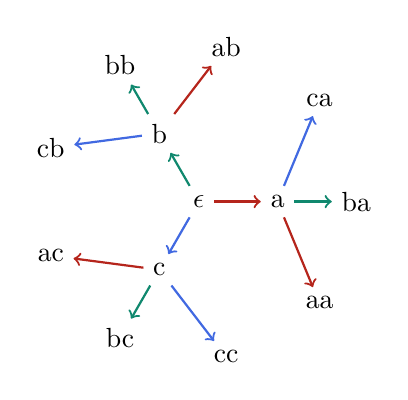
\begin{tikzpicture}
        \node (e) at (0,0) {$\epsilon$};
        \node (a) at (0:1) {a};
        \node (b) at (120:1) {b};
        \node (c) at (240:1) {c};
        \node (aa) at (-40:2) {aa};
        \node (ba) at (0:2) {ba};
        \node (ca) at (40:2) {ca};
        \node (ab) at (80:2) {ab};
        \node (bb) at (120:2) {bb};
        \node (cb) at (160:2) {cb};
        \node (ac) at (200:2) {ac};
        \node (bc) at (240:2) {bc};
        \node (cc) at (280:2) {cc};
    
        \draw[thick,->,BrickRed] (e) -- (a);
        \draw[thick,->,PineGreen] (e) -- (b);
        \draw[thick,->,RoyalBlue] (e) -- (c);
    
        \draw[thick,->,BrickRed] (a) -- (aa);
        \draw[thick,->,PineGreen] (a) -- (ba);
        \draw[thick,->,RoyalBlue] (a) -- (ca);
    
        \draw[thick,->,BrickRed] (b) -- (ab);
        \draw[thick,->,PineGreen] (b) -- (bb);
        \draw[thick,->,RoyalBlue] (b) -- (cb);
    
        \draw[thick,->,BrickRed] (c) -- (ac);
        \draw[thick,->,PineGreen] (c) -- (bc);
        \draw[thick,->,RoyalBlue] (c) -- (cc);
    \end{tikzpicture}
\end{center}
This is another algebra, with one nullary operator 
$\epsilon$ and three unary operators {\color{BrickRed}a$\Box$}, 
{\color{PineGreen}b$\Box$}, and {\color{RoyalBlue}c$\Box$}
being the production rules, that is the tree colors of arrows.

\code{Char:=['a','b',...,'z']}.
\begin{lstlisting}[language=Hidris]
data String = Empty | Prepend( head:Char, tail:String) 
\end{lstlisting}
Writing \lstinline{head:Char} or \lstinline{tail:String} 
indicates that head must come from the alphabet we chose 
and tail must be some already produced string, possibly empty.
Some readers might relate to a different dialect of 
programming such as the following
\begin{lstlisting}[language=Sava]
class String
    case Empty extends String
    case Prepend( head:Char, tail:String) extends String
sealed
\end{lstlisting}
The head here caries around what we put in the list and the tail 
is what comes next in the list.  Observe the similarities:
\begin{align}
     2 & \defeq S(S(0)) \tag{$\mathbb{N}$}\\
 \text{\lstinline{"me"}} & \defeq \text{\lstinline{Prepend('m',Prepend('e',Empty))}}
\tag{String}
\end{align}
The left-hand sides are merely notation for what the data really is on the right.
Both the successor and the \lstinline{Prepend} are operators that generate 
new values.  So part of algebra is to generate new data; so, it is no wonder 
that it closely connections to computation.

\subsection*{Exercise}
\begin{enumerate}
    \item Mimic the String data type to make a list of integers (that is 
    switch from the alphabet to integers).

    \index{generics}
    \item Mimic the String data type to make a list of fixed by 
    unknown data of type $A$, call it \lstinline{List[A]}.\footnote{
    Alternatives include \lstinline{List a} and \lstinline{List<A>}. 
    Search for \emph{generics} in your programming language to learn more.
    }

\end{enumerate}
\index{nil}\index{cons}\index{list}
Historically \lstinline{Empty} for lists is called \lstinline{Nil} 
and \lstinline{Prepend} is called \lstinline{Cons}.



\subsection{Eliminating numbers.}
Now that we have created numbers we shall want to use them.
An obvious use of numbers in counting is to make the process 
modular and parallel.  For example we can have two separate counts 
later combined by addition.
\begin{center}
    \begin{tabular}{c|ccccc}
    ``add'' & \StrokeOne & \StrokeTwo & \StrokeThree & \StrokeFour & \StrokeFive\\
    \hline 
    \StrokeOne & \StrokeTwo & \StrokeThree & \StrokeFour & \StrokeFive & \StrokeOne \StrokeFive\\
    \StrokeTwo & \StrokeThree & \StrokeFour & \StrokeFive & \StrokeOne \StrokeFive & \StrokeTwo \StrokeFive\\
    \StrokeThree & \StrokeFour & \StrokeFive & \StrokeOne \StrokeFive & \StrokeTwo \StrokeFive & \StrokeThree \StrokeFive \\
    \StrokeFour & \StrokeFive & \StrokeOne \StrokeFive & \StrokeTwo \StrokeFive & \StrokeThree \StrokeFive & \StrokeFour \StrokeFive\\
    \StrokeFive & \StrokeOne \StrokeFive & \StrokeTwo \StrokeFive & \StrokeThree \StrokeFive & \StrokeFour \StrokeFive & \StrokeFive \StrokeFive\\
    \end{tabular}
    \hspace{1cm}
    \begin{tabular}{|c|cccccc|}
        \hline 
        + & 0 & 1 & 2 & 3 & 4 & 5\\
        \hline 
        0 & 0 & 1 & 2 & 3 & 4 & 5 \\
        1 & 1 & 2 & 3 & 4 & 5 & 6\\
        2 & 2 & 3 & 4 & 5 & 6 & 7\\
        3 & 3 & 4 & 5 & 6 & 7 & 8\\
        4 & 4 & 5 & 6 & 7 & 8 & 9\\
        5 & 5 & 6 & 7 & 8 & 9 & 10\\
    \hline
    \end{tabular}
\end{center}
Beyond a table we need some formulas.  If we have two groups $m$ and $n$ and each is either nothing 
or a successor to something else, then that leaves us with just four cases 
to consider.
\begin{align*}
    \begin{array}{|c|cc|}
        \hline 
        + & 0 & S(k)\\
        \hline 
        0 & 0 & S(k) \\
        S(\ell) & S(\ell) & S(S(\ell+k))\\
        \hline
    \end{array}
\end{align*}
As the first column does not change $m$ we can simplify this down to 2 cases.
\begin{align*}
    m+n \defeq \begin{cases} m & n=0\\ S(m+k) & n=S(k)\end{cases}
\end{align*}



Addition is different from $S$ because addition is not making new 
numbers, it is actually just refashioning numbers into others.

approach was 
more mathematical than digits and he wrote down 



\newpage

Whatever you understand about mathematics or programs one thing should 
stand out about the nature of $0$, \code{Z}, \code{Zero}, 
$+$, \code{S}, and \code{Next}.  These are not functions.  
That is because each of these is in the service of creating 
numbers, not merely moving them around like a function would.
Zooming in on one of the programs makes this exceptionally noticeable.

\subsection{A closer look}
Perhaps the most convincing way to see that we are creating 
data is to run this process all the way down to what a machine 
must do and witness that somewhere the computer must somewhere 
as for storage space.  We will do this 
in stages as the bottom is a mighty long fall.

A first step might be to convert the cases into a sequence 
of two functions which both make appropriate changes to 
some internal value.  This might look like this:
\begin{center}
\begin{lstlisting}[language=Java]
class NaturalNumber {
    int value // Internal computer storage
    Zero() {value=0} // zero out the memory
    Next(k:NaturalNumber){value=k+1}
}
z = new Zero()  // make a 0
two = new Next(new Next(z)) // make a 2
\end{lstlisting}
\end{center}

Grouping this under a single data type `NaturalNumber'
is mostly just for us not to get confused.  When we 
zoom in closer we find that the computer splits 
this apart, making the storage space separate from the 
functions that use it.  Here is a lower level take
and a realization that indeed both introductions (constructors)
need to ask for some storage, they do not really know 
how much, the computer calculates that for them.
\begin{center}
\begin{lstlisting}[language=C]
struct Nat { int length, uint8[] digits }
Nat NaturalNumber_Zero() { 
    memory = malloc(Nat) // allocate memory
    memory.length = 1
    memory.value[0] = 0
    return memory 
}
Nat NaturalNumber_Next(k:Nat) {
    memory = malloc(Nat) // allocate memory
    if k.digits[k.length-1] != 0 then
        memory.length = length +1
    
    memory.digits = k.digits +1
    return memory 
}
\end{lstlisting}
\end{center}

If we zoom in even further we see this `malloc' command eventually 
translate into asking for actual memory in the computer.  Here is a
simplified take that assumes the length is fixed at 9 bytes, that is 
the maximum value reached is $2^{128}$, it would take all the computers 
in the world to tally from $0$ to $2^{128}$ in your lifetime so 
this is a safe limit.
\begin{center}
\begin{lstlisting}[language={ [x86masm]Assembler}]
%macro NaturalNumber_Zero 0
    mov param1, 0x0009      ; move 4 into first parameter
    call malloc            ; storage of size param1 (=9)
    mov store, 0x0000      ; mov 0 into the storage
    ret 

%macro NaturalNumber_Next 1
    int  temp
    mov  temp, param1     ; make a copy of first input
    mov param1, 0x0009      
    call malloc          ; storage of size 9
    mov  store, temp     ; move input to storage
    inc  store           ; increment storage 
    ret 
\end{lstlisting}
\end{center}

As this snippet reveals this program comes to a physical limit 
once we exceed the internal storage capabilities of integers in the
system.  We can fix this but the spirit of the programs above 
is to separate the need to understand the computer deeply and see the 
overall behavior.



If we hold on only to these ideas then we are narrowing what we need 
to know about natural numbers to just some fixed rules, so far the rules 
on how to create them.  So let us say that the symbol $\mathbb{N}$ represents 
all the rules that apply to natural numbers and that writing $0:\mathbb{N}$ or 
$n:\mathbb{N}$ is a way of saying that the symbols $0$ and $n$ obey those rules.
Using $\vdash$ to mean  ``yields'', 
In other words
\begin{description}
    \item[Zero] $\vdash 0: \mathbb{N}$, nothing is need to  yield $0$ as a natural number.
    \item[Successor] $k:\mathbb{N}\vdash S(k):\mathbb{N}$, every natural number  $k$ yields 
    another $S(k)$.
\end{description}
We can get back to childhood 
counting by giving names to these Peano numerals
\begin{center}
    $0\defeq 0$,
    $1\defeq S(0)$,
    $2\defeq S(S(0))$,
    $3\defeq S(S(S(0)))$,...
\end{center}
The point is, the successors are not so much a function 
moving around the numbers that we find laying around, it
\emph{makes} numbers.  
If it were not it would not continue forever 
and what would `$\ldots$' and `etc.' mean in your mind?

\subsection{Computational significance.}
Just as we switched Peano's $a+$ to $S(k)$;
it would be no serious issue to have used $a++$, $++a$, or \lstinline{next k}.
Programmers today use a number of alternatives to encode natural 
numbers.  Some languages hold close to mathematical notation 
preferring symbols to have meaning, like the following formula:
\begin{center}
\begin{lstlisting}[language=Hidris]
    data Nat = Z:Nat | S (k:Nat)
\end{lstlisting}
\end{center}
Whatever ``data'' does we can assume it make the computer see what comes 
next as describing a new type of data, `Nat'.  And the symbols 
$Z$ and $S k$ are distributed into cases separated by `|'.

Other languages face business and industry and package data 
verbosely to help communicate the meaning, for example:
\begin{center}
\begin{lstlisting}[language=Sava]
class NaturalNumber
    case Zero extends NaturalNumber
    case Next(k:NaturalNumber) extends NaturalNumber
sealed  // no more cases
\end{lstlisting}
\end{center}
Words like ``data'', ``class'', ``case'' and ``sealed'' are 
called keywords and usually show up in different colors just to make 
sure we notice they have special roles to play in the language.
A successful programming language (PL) will choose keywords 
that have some reasonable ``obvious meaning''.  This means that you 
can learn to read code in most languages by scanning for patterns 
and using keywords as clues to tie the meaning together.  Take 
a moment to see that you see Peano's main idea in both of the above 
code fragments.

\begin{definition}
    In logic rules that explain what produces a symbol are called 
    \emph{introductions}, e.g.\ $\vdash 0:\mathbb{N}$ and 
    $k:\mathbb{N}\vdash S(k):\mathbb{N}$ are introduction rules.
    
    In programming the word \emph{constructor} is often preferred
    as it explains how to construct data of a specified type.        
\end{definition}

\subsection{Reaching new uses.}

The point of basic patterns is to use them in more complex systems
with an understanding of the resulting behavior.  Imagine a string 
of characters in an alphabet \lstinline{Char:=['a','b',...,'z']}.
\begin{lstlisting}[language=Hidris]
data String = Empty | Prepend( head:Char, tail:String) 
\end{lstlisting}
Writing \lstinline{head:Char} or \lstinline{tail:String} 
indicates that head must come from the alphabet we chose 
and tail must be some already produced string, possibly empty.
Some readers might relate to a different dialect of 
programming such as the following
\begin{lstlisting}[language=Sava]
class String
    case Empty extends String
    case Prepend( head:Char, tail:String) extends String
sealed
\end{lstlisting}
The head here caries around what we put in the list and the tail 
is what comes next in the list.  Observe the similarities:
\begin{align}
     2 & \defeq S(S(0)) \tag{$\mathbb{N}$}\\
 \text{\lstinline{"me"}} & \defeq \text{\lstinline{Prepend('m',Prepend('e',Empty))}}
\tag{String}
\end{align}
The left-hand sides are merely notation for what the data really is on the right.
Both the successor and the \lstinline{Prepend} are operators that generate 
new values.  So part of algebra is to generate new data; so, it is no wonder 
that it closely connections to computation.

\subsection*{Exercise}
\begin{enumerate}
    \item Mimic the String data type to make a list of integers (that is 
    switch from the alphabet to integers).

    \index{generics}
    \item Mimic the String data type to make a list of fixed by 
    unknown data of type $A$, call it \lstinline{List[A]}.\footnote{
    Alternatives include \lstinline{List a} and \lstinline{List<A>}. 
    Search for \emph{generics} in your programming language to learn more.
    }

\end{enumerate}
\index{nil}\index{cons}\index{list}
Historically \lstinline{Empty} for lists is called \lstinline{Nil} 
and \lstinline{Prepend} is called \lstinline{Cons}.



